O conceito de jogos de tiro multijogador em que cada jogador controla personagens de classes diferentes ou heróis totalmente únicos se popularizou em jogos mais recentes, como Team Fortress 2 (2007) \footnote{Team Fortress 2: jogo de tiro em primeira pessoa desenvolvido pelo estúdio Valve , em 2007}, os jogos da série Battlefield , Overwatch (2016) e Paladins (2018).
Tanto Paladins quanto Overwatch se assemelham ao jogo proposto pelo trabalho pois são jogos multiplayer de tiro em primeira pessoa com mapas compactos e movimentação rápida, contudo os jogos citados priorizam mais a assimetria de jogabilidade, com personagens únicos.

\begin{figure}[htb]
    \caption{\textit{Hero shooters} modernos} 
	\label{fig:jogosSimilaresModernos}
	\centering
	\subfloat[Paladins]{
		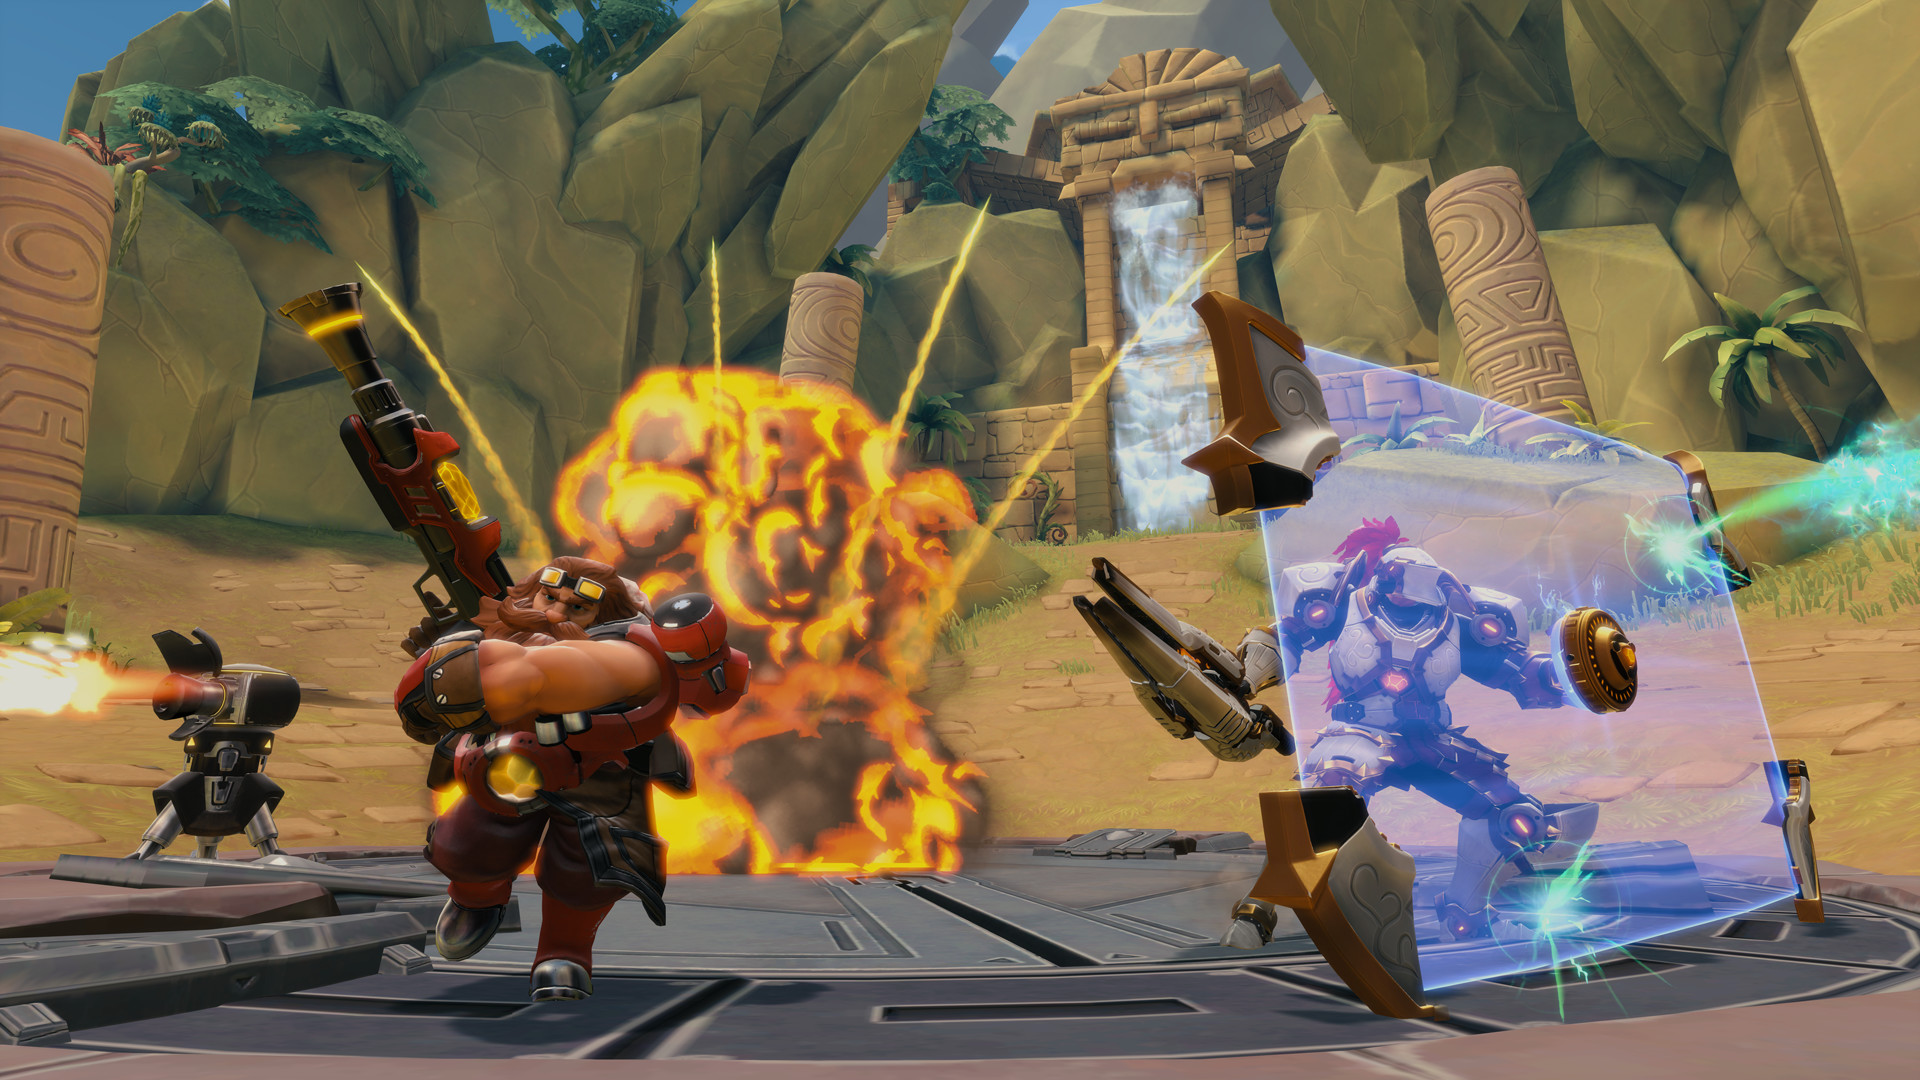
\includegraphics[scale=0.1]{imgs/paladins.jpg}
	}\hspace{0.15cm} 
	\subfloat[Overwatch]{
		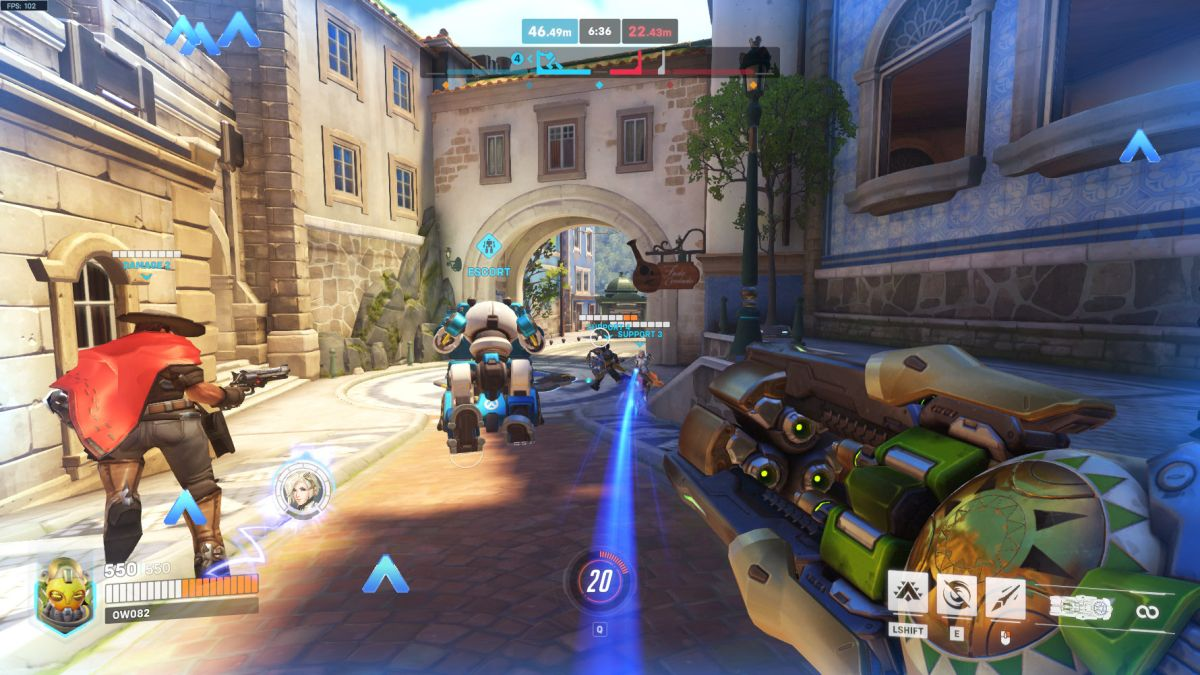
\includegraphics[scale=0.15]{imgs/overwatch.jpeg}
	}
	%redimensionar as imagens ?
	%\fonte{}
    %https://criticalhits.com.br/games/paladins-sera-lancado-para-consoles/
    %https://pt.jugomobile.com/revisao-de-overwatch-2/
    
\end{figure}

A análise histórica dos gêneros que compõem o jogo proposto desempenha um papel fundamental na definição da visão e mecânicas do nosso projeto. Inspirados por precursores notáveis, como DOOM, que popularizou os jogos de tiro em primeira pessoa 3D, e pelos emblemáticos Quake III Arena e Unreal Tournament, que estabeleceram os alicerces do 'arena shooter', nosso jogo se esforça para capturar a essência dessas experiências clássicas. Os elementos competitivos e ação intensa característicos dos jogos de arena se tornaram a base de nossa proposta, onde os jogadores enfrentarão desafios em mapas compactos, com foco na habilidade individual e estratégias táticas. Além disso, a influência desses gêneros se estende à variedade de modos de jogo e à ênfase na jogabilidade multiplayer, proporcionando aos jogadores uma experiência de jogo envolvente e dinâmica.


, tal ato é conhecido como "screen cheating", uma forma de trapacear em jogos de tela dividida em que saber a posição do outro jogador oferece alguma vantagem, como em jogos de tiro)